\chapter{Additional Details for Michel Electron Reconstruction}\label{ch:energyfits}

\minitoc

Chapter \ref{ch:michel} provided a study of the fractional energy resolution of
the developed Michel electron reconstruction algorithm, in terms of ionisation
only deposited energy. The bias and resolution estimates were based on
gaussian fits to the fractional difference between the reconstructed ionisation
energy and the true ionisation energy. The fits used to populate Figure
\ref{fig:res_and_bias_ion} are shown in Figure \ref{fig:ionisation_fits}. The 
data is binned in terms of the total true ionisation energy deposited by the 
Michel electron, and each plot contains the data from a single bin. No attempt 
was made to fit the tails of the distribution, which is particularly 
noteworthy in Figure \ref{fig:ion_fit_30}, where there is a significant tail 
for negative fractional differences. 

\begin{figure}

	\centering
	\begin{subfigure}[b]{0.49\textwidth}
		\centering
		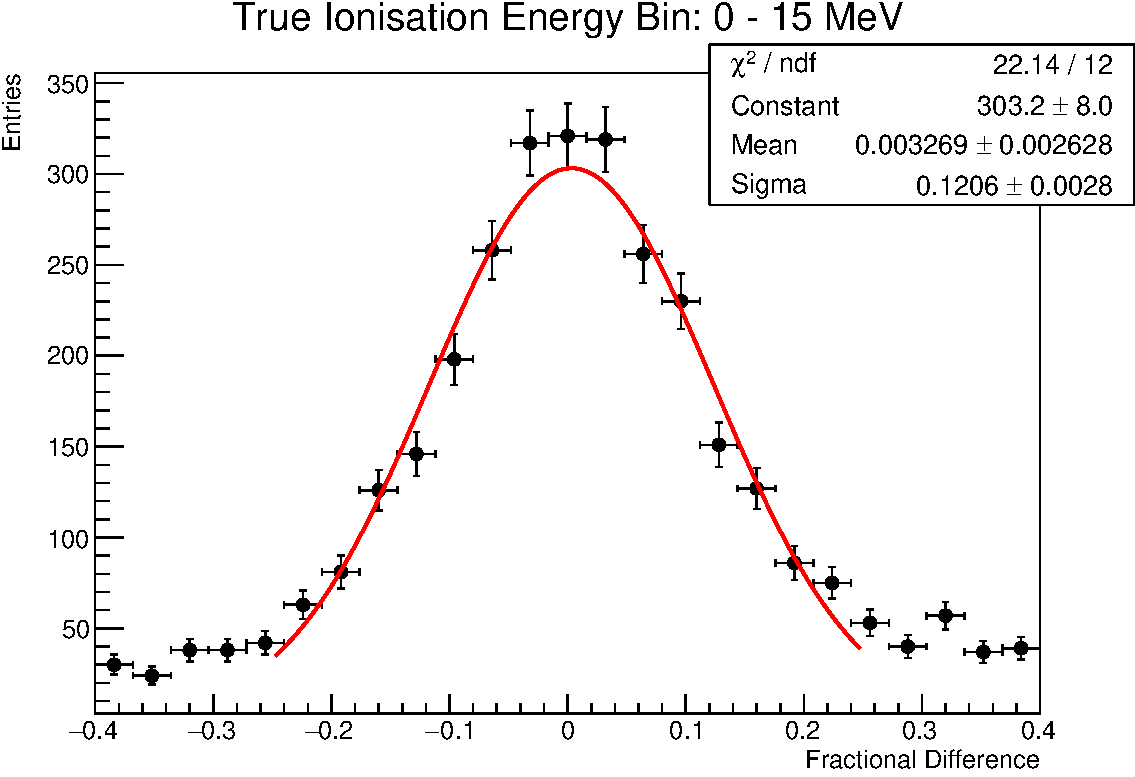
\includegraphics[width=\textwidth]{figures/ion_res_0.pdf}
		\caption {0 - 15 MeV}
	\end{subfigure}
	\hfill
	\begin{subfigure}[b]{0.49\textwidth}
		\centering
		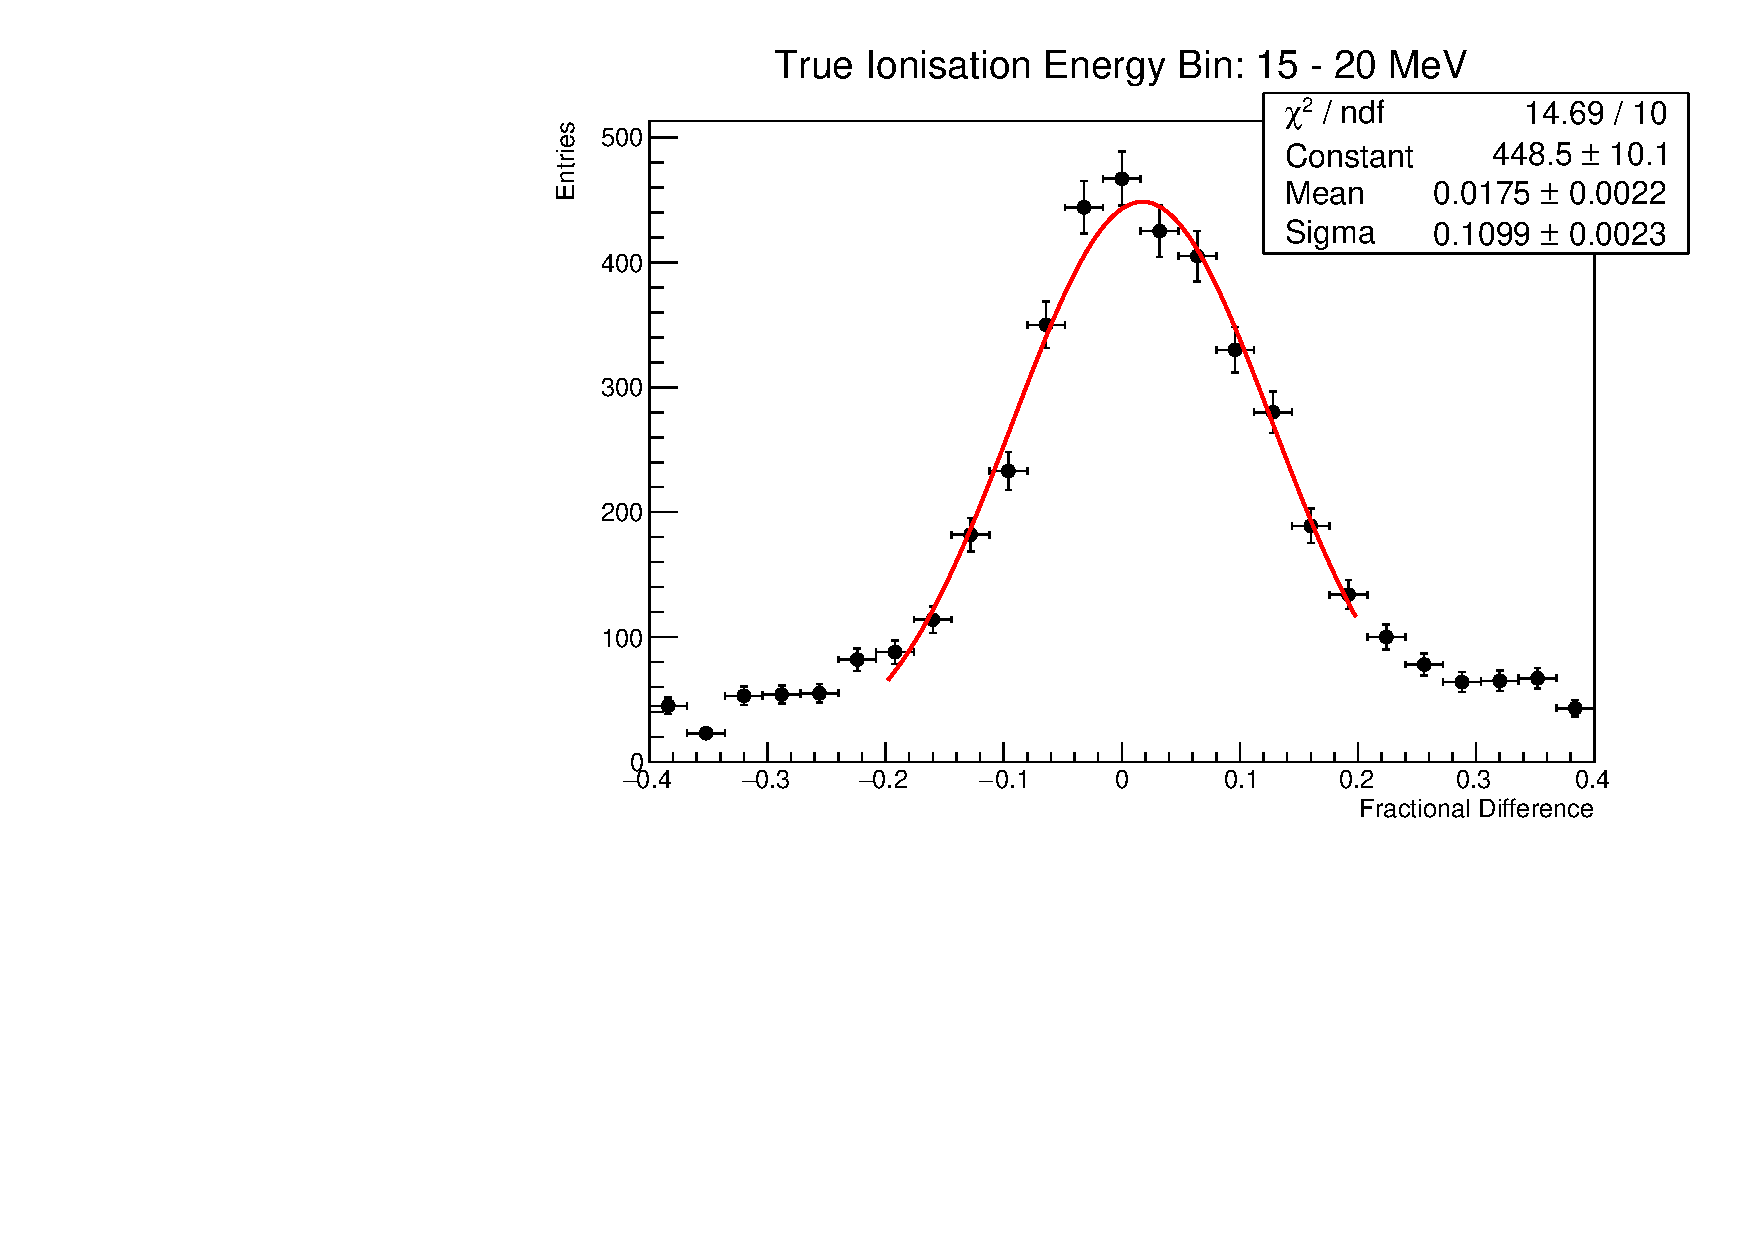
\includegraphics[width=\textwidth]{figures/ion_res_15.pdf}
		\caption {15 - 20 MeV}
	\end{subfigure}
	\begin{subfigure}[b]{0.49\textwidth}
		\centering
		\vspace{5mm}
		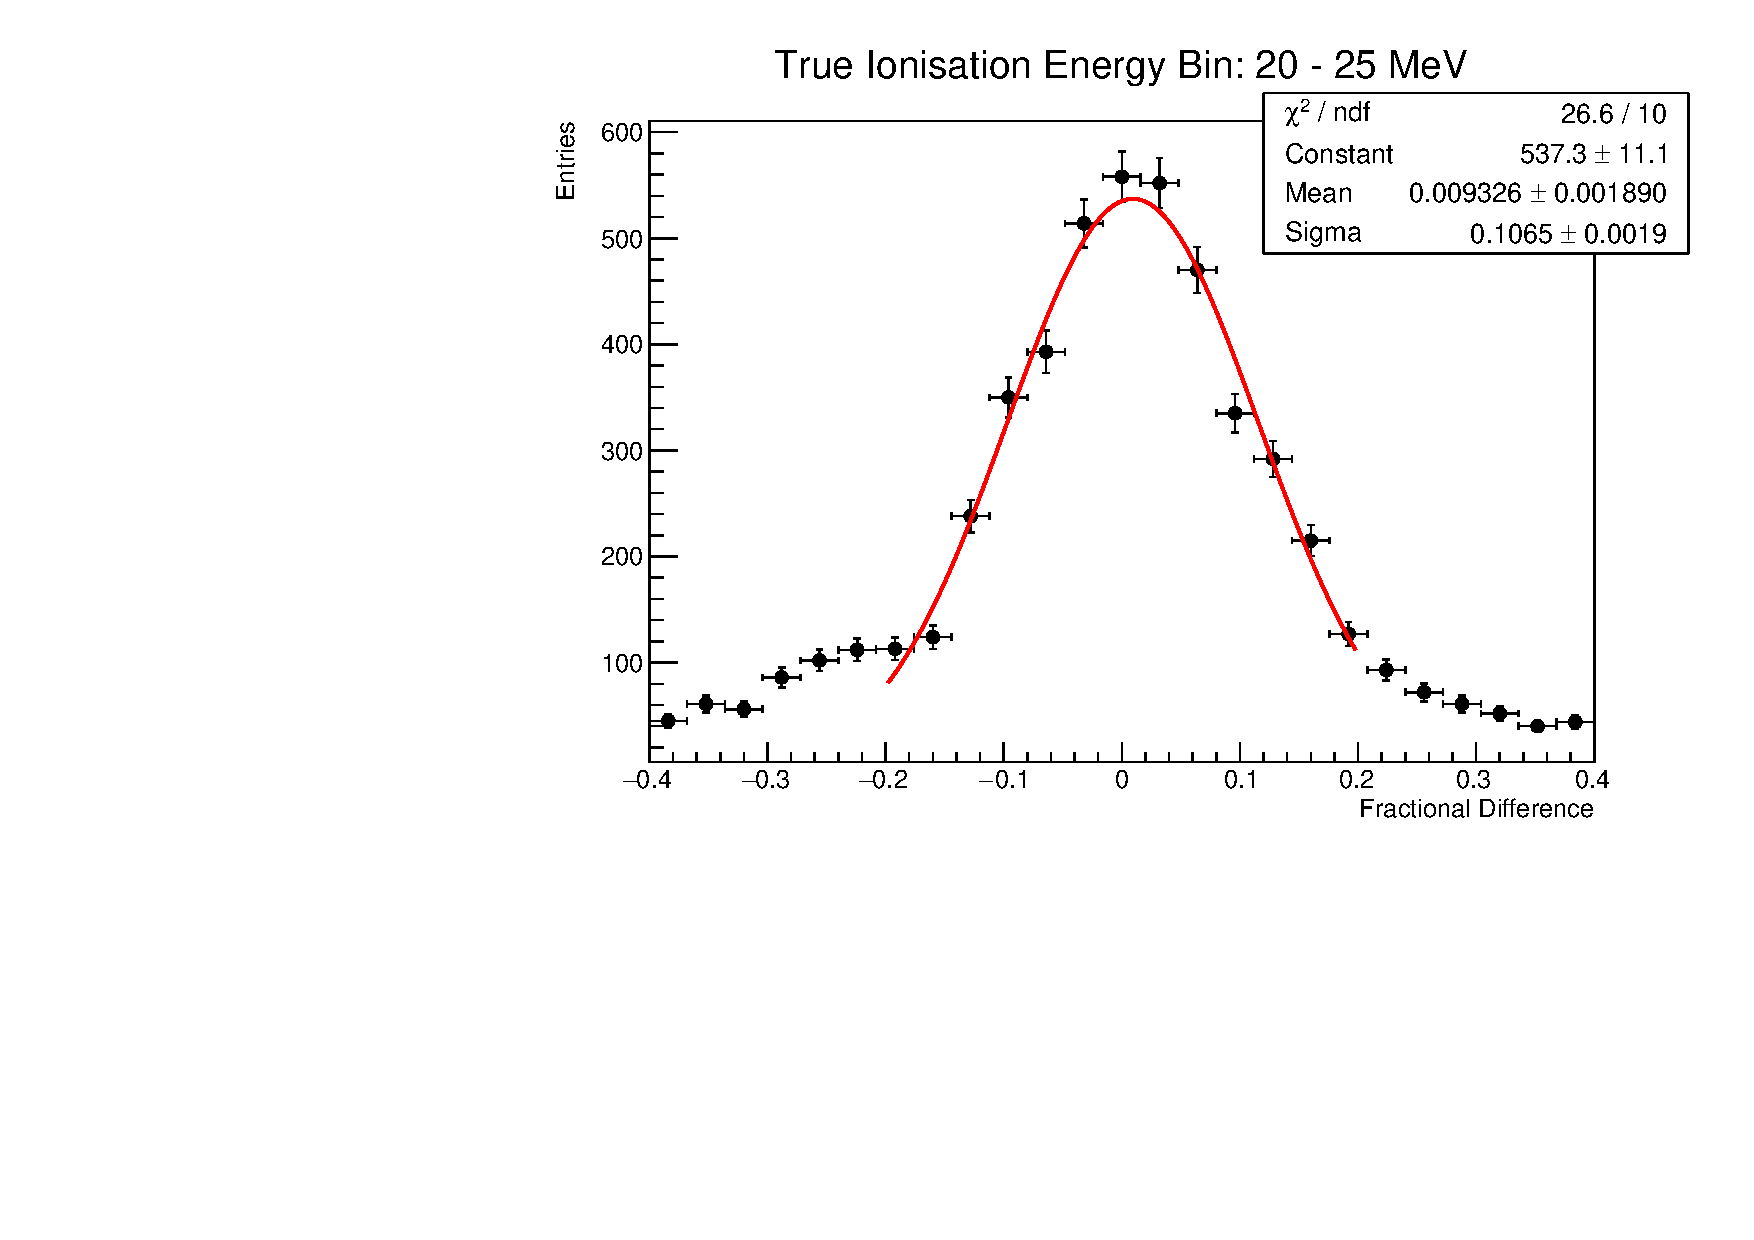
\includegraphics[width=\textwidth]{figures/ion_res_20.pdf}
		\caption {20 - 25 MeV}
	\end{subfigure}
	\hfill
	\begin{subfigure}[b]{0.49\textwidth}
		\centering
		\vspace{5mm}
		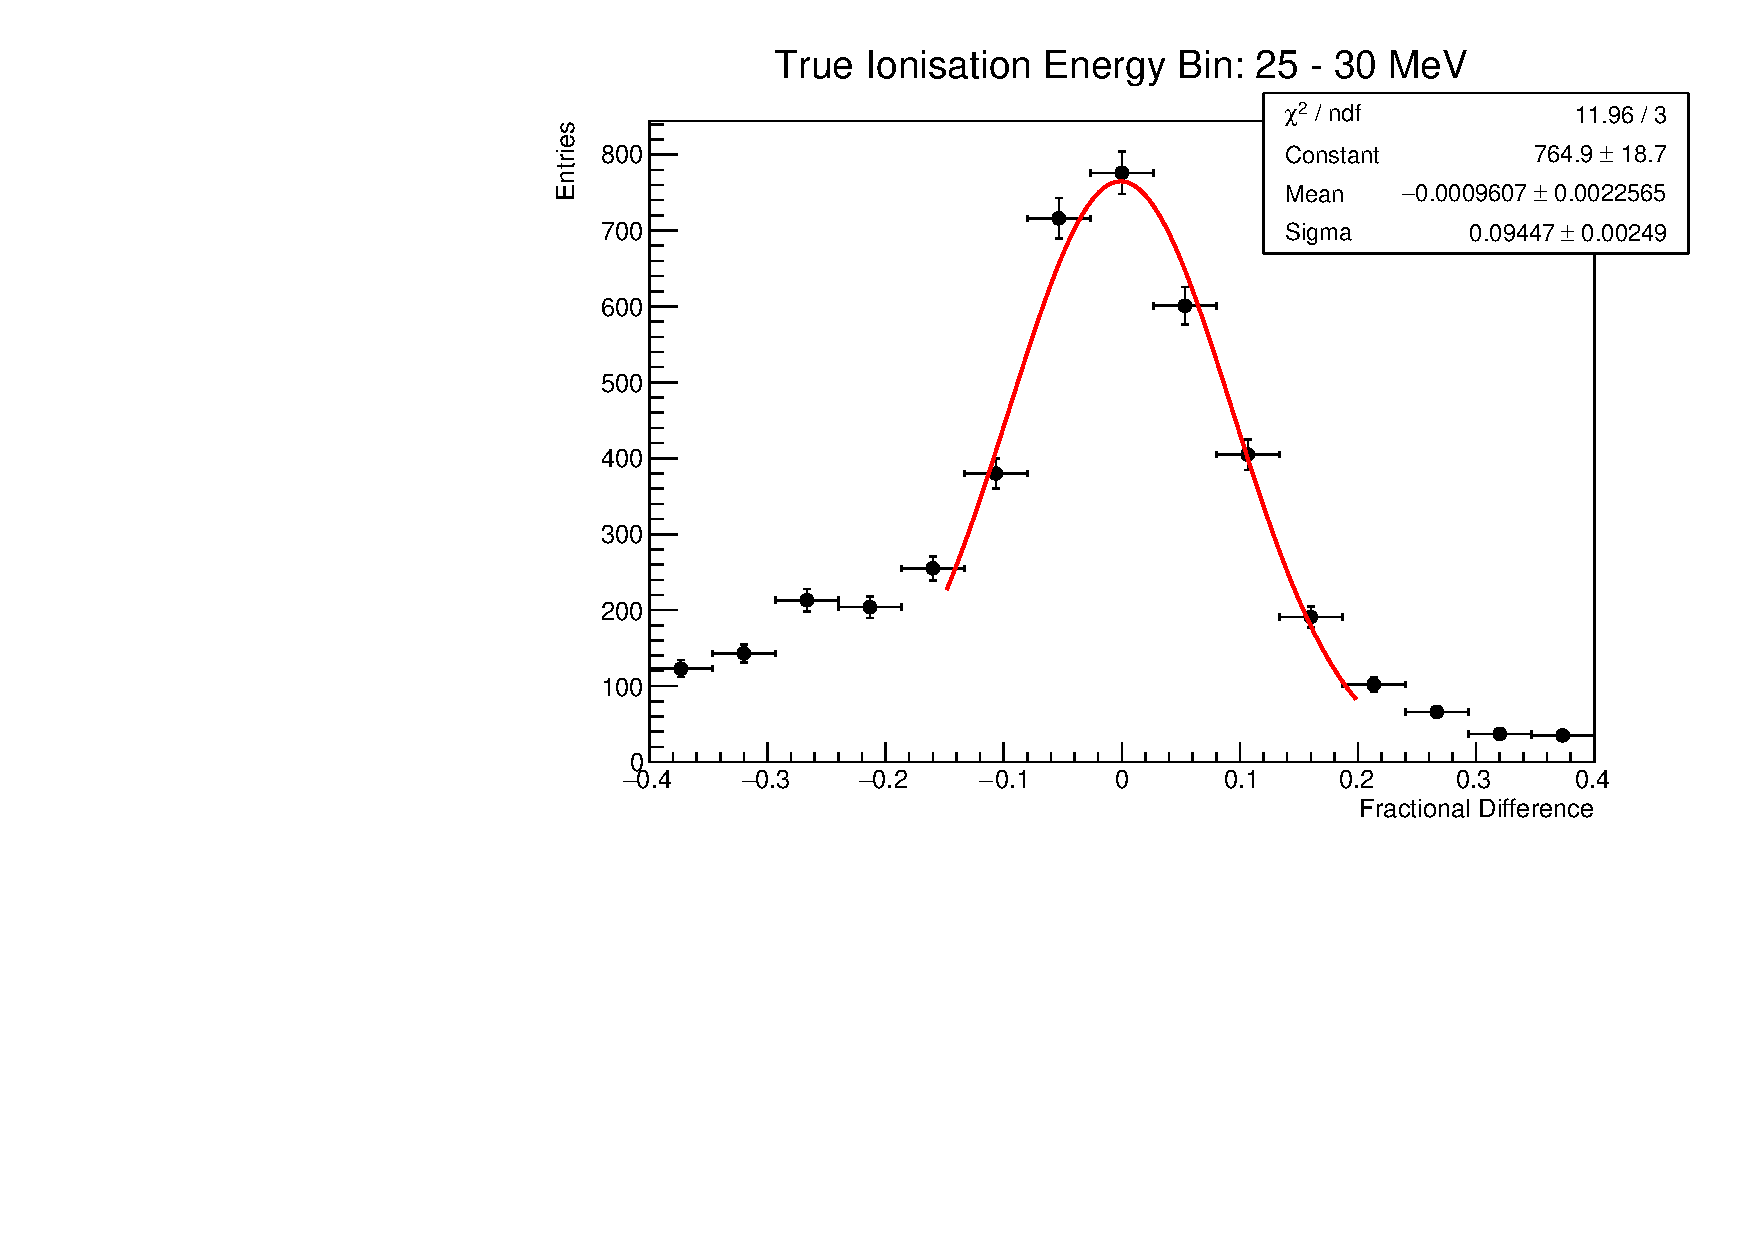
\includegraphics[width=\textwidth]{figures/ion_res_25.pdf}
		\caption {25 - 30 MeV}
	\end{subfigure}
	\begin{subfigure}[b]{0.49\textwidth}
		\centering
		\vspace{5mm}
		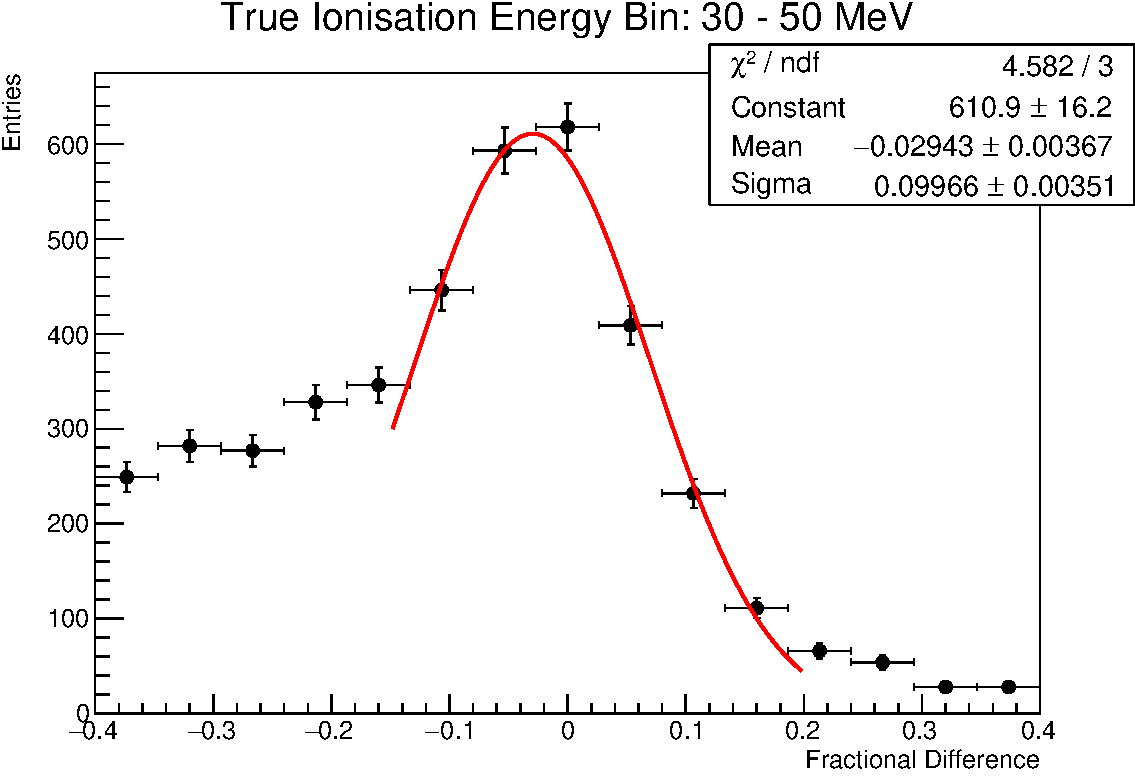
\includegraphics[width=\textwidth]{figures/ion_res_30.pdf}
		\caption {30 - 50 MeV}
		\label{fig:ion_fit_30}
	\end{subfigure}

	\caption
	[Gaussian fits to the fractional energy difference bewteen the reconstructed
	ionisation energy and the true ionisation energy for Michel electron events.]
	{Gaussian fits to the fractional energy difference between reconstructed 
	ionisation energy and true ionisation energy, used to estimate the energy 
	resolution and bias as a function of energy in Figure 
	\ref{fig:res_and_bias_ion}. No Attempt was made to fit the tails of the 
	distribution.}
	\label{fig:ionisation_fits}

\end{figure}
